\section{Agent Communication}
Agent communication is one of the cornerstones of multi-agent systems. Since each agent is autonomous and features goal-driven behaviour, the overall communication mechanism is much more ``human-like'': instead of executing requests, it becomes more of a deal-making utility-centered conversation. But for that conversation to exist agents at least should understand each other. To make it easier to design the agent communication, different agent communication languages were created. The most popular are FIPA-ACL, KQML and KIF \cite{ap5, DUMMY:1,DUMMY:2,DUMMY:3}.
\subsection{KQML}
KQML stands for Knowledge Query and Manipulation Language.
This language represents a message as an object. Each message has a performative that specifies its type and a list of parameters, which are depicted as ``attribute:value'' pairs.
\begin{center}
\begin{tabular}{|p{1cm} |p{3cm} | p{12cm}|}
\multicolumn{3}{c}{\textbf{Some attributes of KQML}}\\
\hline
\textnumero & \textbf{attribute} & \textbf{meaning} \\
\hline
1&:content    & content of the message \\
\hline
2&:force      & whether the sender of the message will ever deny the content of the message \\
\hline
3&:in-reply   & whether the sender expects a reply, and, if so, an identifier for the reply \\
\hline
4&:reply-with & adding the preferable response specification. \\
\hline
5&:sender     & sender of the message \\
\hline
6&:receiver   & intended recipient of the message\\
\hline
\end{tabular}
\newline
\end{center}
Therefore, a message in KQML may look like this one:
\begin{align*}
(\ & \text{ask-one} \\
  &:content\ (COLOR\ GNOMEHAT\ ?\ color) \\
  &:receiver\ tailor                    \\
  &:language\ LPROLOG                   \\
  &:ontology\ gnome-info\ )             \\
\end{align*}

 ``Ask-one'', in the message above, is a performative. There are around 50 performatives in KQML, each describing the corresponding message type.\par
 The dialogues in KQML can be either synchronous or asynchronous. The types of dialogues are represented on Figure~\ref{KQMLDialog}.
    \begin{figure}[h!]
      \begin{center}
     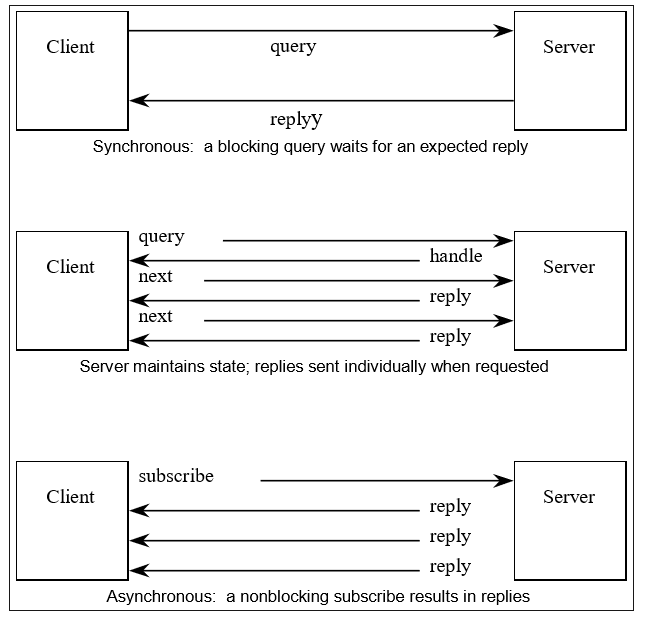
\includegraphics[width=300pt]{kqml}
      \caption{BDI agent architecture.}
      \label{KQMLDialog}
      \end{center}
    \end{figure}

\subsection{FIPA}
Since FIPA ACL was designed for the same purposes as KQML, this two languages have much in common.
The goal behind the creation of the FIPA standard is to utilize it in the development of an agent communication language (FIPA-ACL).  FIPA-ACL is superficially similar to KQML: it defines an ``outer'' language for messages, feature 20 performatives for defining the intended interpretation of messages, and it does not mandate any specific language for message content. In addition, the concrete syntax for FIPA-ACL messages closely resembles that of KQML. For example,the example KQML message from above when encrypted in FIPA-ACL using XML markup language is presented below:
\addtolength{\jot}{-10pt}
\begin{align*}
  &<\text{envelope}> \\
  &\quad <\text{params} index ="1"> \\
  &\quad \quad <\text{to}> \\
  &\quad \quad \quad <\text{agent-identifier}>\\
  &\quad \quad \quad \quad <\text{name}> tailor </\text{name}>\\
  &\quad \quad \quad </\text{agent-identifier}>\\
  &\quad \quad </\text{to}> \\
  &\quad \quad <\text{from}> \\
  &\quad \quad \quad ... \\
  &\quad \quad </\text{from}> \\
  &\quad \quad ...\\
  &\quad </\text{params}>\\
  &</\text{envelope}>\\
  &</\text{message}>\\
  &\quad </\text{performative}>\\
  &\quad \quad ask-one \\
  &\quad </\text{performative}>\\
  &\quad </\text{content}>\\
  &\quad \quad ? \\
  &\quad </\text{content}>\\
  &\quad <\text{ontology}>\\
  &\quad \quad gnome-info \\
  &\quad </\text{ontology}>\\
  &\quad ...\\
  &</\text{message}>\\
\end{align*}

\subsection{KIF}
The knowledge interchange format (KIF) is a simple logic-based language that gained high popularity in  expert systems, databases and intelligent agents. The initial design objective of KIF was to create a ``mediator'' language, useful for translating messages between other languages. The simple example featuring this language is given below.
\begin{center}
\textit{(> (- (length sword) (shaftLength sword)) (- (length knife) (shaftLength knife))) }
\end{center}
This example states that the sword has the longer blade than the knife does.
Despite the existence of this communication protocols there are a lot of cases where it is much more rewarding to create personalized communication protocol for a particular system. However, KQML or FIPA-compliance can make a multi-agent system easily understandable and mergeable with others.
